\documentclass[a4paper,twocolumn]{article}

\RequirePackage[croatian]{babel}
\makeatletter
\renewcommand\thesection{\@arabic\c@section.}
\renewcommand\thesubsection{\thesection\@arabic\c@subsection.}
\renewcommand\thesubsubsection{\thesubsection\@arabic\c@subsubsection.}
\renewcommand\theequation{\@arabic\c@equation}
\renewcommand\thefigure{\@arabic\c@figure.}
\renewcommand\thetable{\@arabic\c@table.}
\makeatother

\RequirePackage{graphicx}
\RequirePackage{hyperref}
\RequirePackage{amssymb}
\RequirePackage{amsmath}
\RequirePackage{booktabs}

\title{Raspoznavanje znakova znakovnog jezika}
\author{Lucija Čorak, Mateo Jakšić, Petar Kuruc, Martina Šola, Klara Zagajski}
\date{}

\begin{document}

\maketitle


\section{Uvod}

Znakovni jezik predstavlja osnovno sredstvo komunikacije za gluhe i nagluhe osobe. Automatizirano prepoznavanje znakova znakovnog omogućuje bolju integraciju gluhih osoba u svakodnevni život.


U okviru ovog rada razvijen je i evaluiran sustav za automatsko prepoznavanje znakova znakovnog jezika temeljen na metodama dubokog učenja.

Radimo klasifikaciju na CNN i ResNet modelima na sljedećim skupovima podataka:
\begin{itemize}
    \item \textbf{Originalne slike ($28 \times 28$):} 
    izvode se na originalnim slikama dimenzija ($28 \times 28$).
    \item \textbf{Izjednačeni histogrami ($28 \times 28$):} izvode se na slikama nakon izjednačavanja histograma, zadržavajući rezoluciju ($28 \times 28$).
    \item \textbf{x2 super-rezolucija ($112 \times 112$):}  izvode se na slikama povećanim na ($112 \times 112$) piksela korištenjem x2 super-rezolucije.
    \item \textbf{x4 super-rezolucija ($112 \times 112$):}  izvode se na slikama povećanim na ($112 \times 112$) piksela korištenjem x4 super-rezolucije.
\end{itemize}



\section{Korišteni skup podataka}

Korišten je javno dostupan skup podataka znakova američkog znakovnog jezika (ASL), koji se sastoji od slika koje prikazuju ruke u različitim pozicijama koje odgovaraju slovima engleske abecede. Skup je podijeljen na dijelove za treniranje i testiranje.

Skup podataka dostupan je na platformi Kaggle te je referenciran kao \cite{asl_dataset}.

Radi se o slikama dimenzije ($28 \times 28$) piksela u sivim tonovima, a svaka slika prikazuje jednu gestu koja odgovara slovu engleske abecede (osim slova \textbf{J} i \textbf{Z}, koja uključuju pokret i nisu zastupljena u ovom skupu podataka). Slike su raspoređene u 24 klase, a podatci su formatirani u obliku CSV datoteka, odvojeno na skupove za treniranje i testiranje. Veličina svake slike iznosi 784 piksela.

Podaci su raspodijeljeni na sljedeći način:
\begin{itemize}
    \item Trening skup: 27\,455 uzoraka
    \item Testni skup: 7\,172 uzoraka
\end{itemize}

Originalno, postojalo je samo 1\,704 fotografija ruku u boji, nakon čega su primijenjene razne metode kako bi se skup podataka proširio. Dio slike na koje je ruka je izdvojen iz pozadine, skaliran na ($28 \times 28$), pretvoren u sive tonove i zatim su primijenjene transformacije. One su uključivale 5\% nasumičnu pikselaciju, $\pm 15$\% promjenu svjetline i kontrasta, rotaciju od $\pm 3^\circ$ i različite filtere (``Mitchell'', ``Spline'', itd.). Time je dobiven veliki broj varijacija svakog znakovnog slova kako bi se poboljšala raznolikost i izazovnost klasifikacije \cite{asl_dataset}.



\section{Obrada slike}

Prije treniranja modela provedena je obrada ulaznih slika kako bi se poboljšala kvaliteta podataka i omogućila robusnost modela. Vrijednosti piksela su normalizirane na raspon [0, 1].



\subsection{Poboljšanje kontrasta (izjednačavanje histograma)}

U pokušaju da se poboljšaju rezultati klasifikacije, primijenjen je postupak izjednačavanja histograma kojim se poboljšava kontrast slike tako da se pikseli rasporede ravnomjernije po čitavom rasponu intenziteta. Dakle, za svaku pojedinačnu sliku računa se kumulativna distribucijska funkcija (CDF) i pripadajuće središnje vrijednosti \emph{binova} pomoću funkcije \texttt{skimage.exposure.cumulative\_distribution}. Zatim se slika transformira interpolacijom - pikseli se preslikavaju tako da rezultat ima ravnomjernije raspoređene intenzitete, te se dobiveni rezultat pretvara u 8-bitni format kako bi ostao u istom formatu kao i original.




Histogramsko izjednačavanje je korisno jer povećava kontrast slika, što zauzvrat može olakšati prepoznavanje rubova i značajki na slikama, a primjer dobivenih rezultata je vidljiv na slici \ref{fig:histogram_D}

\begin{figure}[ht]
\centering
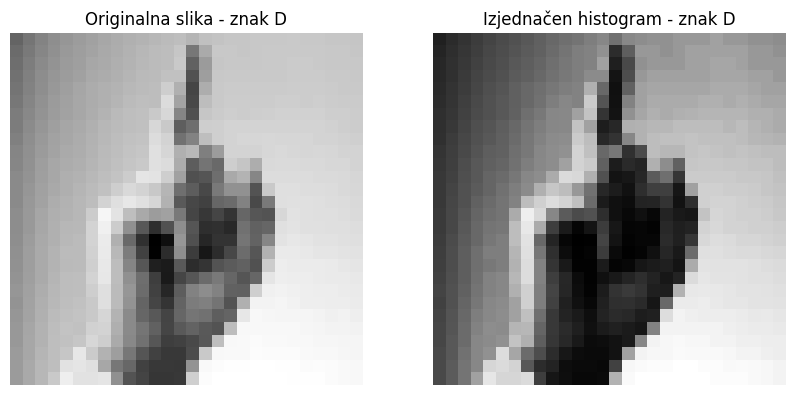
\includegraphics[width=1\linewidth]{compare_histogram_D.png}
\caption{Usporedba originalne slike sa slikom dobivenom nakon izjednačavanja histograma}
\label{fig:histogram_D}
\end{figure}

\subsection{Interpolacija (super rezolucija)}

Cilj interpolacije je povećanje dimenzionalnosti slike. Pošto su slike u korištenom skupu podataka niske rezolucije (28 x 28), postoji nedostatak detalja i oštrine, pa može doći do problema prilikom treniranja. Super rezolucija može pomoći modelima u prepoznavanju finijih detalja ruke i prstiju kod znakovnih jezika, a originalne slike su vrlo malih dimenzija i mogu sadržavati malo vizualnih informacija. To može biti posebno korisno kod korištenja modela poput ResNeta, koji je obično treniran na slikama visoke rezolucije.

\begin{figure}[ht]
\centering
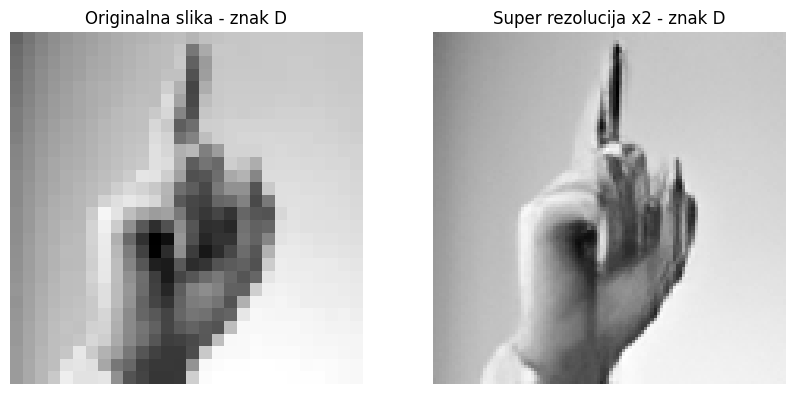
\includegraphics[width=1\linewidth]{compare_super2.png}
\caption{Usporedba originalne slike sa slikom dobivenom nakon super rezolucije ×2}
\label{fig:super2}
\end{figure}

Za potrebe ovog seminara korišten je ESRGAN (Enhanced Super Resolution Generative Adversarial Networks), duboki generativni pretrenirani modeli neuronske mreže koji služe za pametno povećanje rezolucije slika. Navedeni modeli preuzetu su s izvora \cite{RealESRGAN}.

Korištene su dvije vrste skaliranja, skaliranje x2 (slika \ref{fig:super2}) i skaliranje x4 (slika \ref{fig:super4}).


\begin{figure}[ht]
\centering
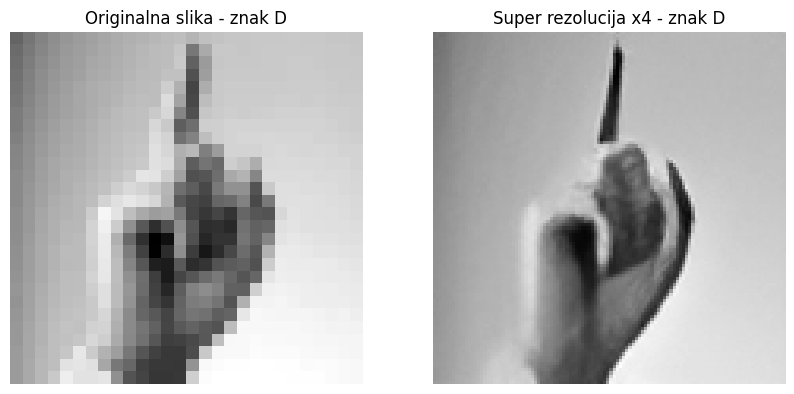
\includegraphics[width=1\linewidth]{compare_super4.png}
s\caption{Usporedba originalne slike sa slikom dobivenom nakon super rezolucije ×4}
\label{fig:super4}
\end{figure}


\section{Modeli}

U svrhu klasifikacije gesti znakovnog jezika korištena su dva tipa modela dubokih konvolucijskih neuronskih mreža, izrađena u Keras/TensorFlow okruženju. Prvi tip modela je klasični konvolucijski neuronski model (CNN), dok drugi implementira rezidualne blokove inspirirane ResNet arhitekturom.

Modeli su razvijeni i trenirani u dvije varijante: za slike izvorne rezolucije ($28 \times 28$) piksela u nijansama sive te za slike proširene na ($112 \times 112$) piksela korištenjem ESRGAN metode super-rezolucije. Cilj je bio klasificirati geste u 24 klase (sve osim slova J i Z koja se temelje na pokretu i nisu prikladna za statičku klasifikaciju).

\subsection{Konvolucijska neuronska mreža (CNN)}

Prva arhitektura temelji se na jednostavnoj hijerarhiji konvolucijskih i potpuno povezanih slojeva. U verziji za ulazne slike veličine ($28 \times 28$), arhitektura se sastoji od dva konvolucijska sloja (s 32 i 64 filtara) s funkcijom aktivacije ReLU, svaki praćen slojem za maksimalno spajanje (engl. MaxPooling2D). Na taj se način smanjuje prostorna dimenzionalnost značajki. Nakon tih slojeva, podaci se "spljošte" (engl. Flatten) i prolaze kroz potpuno povezani sloj sa 128 neurona i ReLU aktivacijom. Naposljetku, podaci prolaze kroz završni izlazni sloj s 24 neurona i softmax aktivacijom za višeklasnu klasifikaciju.

Ova arhitektura jednostavna je za implementaciju i efikasna pri radu s malim skupovima podataka, ali nema mehanizme za ublažavanje problema degradacije performansi s dubinom, za razliku od ResNet-a.

Za treniranje na slikama proširene rezolucije ($112 \times 112$), razvijena je proširena varijanta CNN-a koja uključuje četiri konvolucijska sloja (s 32, 64, 128 i 256 filtara), svaki sa slojem MaxPooling2D. Time se omogućuje izdvajanje složenijih značajki koje postaju dostupne u višoj rezoluciji. Na kraju, koriste se flatten sloj, jedan potpuno povezani sloj s 256 neurona te izlazni softmax sloj.

\subsection{Rezidualna neuronska mreža (ResNet)}

Drugi model uvodi rezidualno učenje pomoću tzv. residual blocks – temeljne ideje ResNet arhitekture. Na ulazu se koristi konvolucijski sloj s 32 filtra, a zatim slijede tri skupine rezidualnih blokova:

\begin{itemize}
\item dvije iteracije bloka s 32 filtra bez promjene dimenzija,
\item dvije iteracije bloka s 64 filtra sa smanjenjem dimenzija (stride=2),
\item dvije iteracije bloka s 128 filtra uz daljnje smanjenje dimenzija.
\end{itemize}

Kako bi se model mogao koristiti za slike dimenzija ($112 \times 112$), proširuje se arhitektura. Dodaje se dodatna grupa blokova s 256 filtra i dodatnim smanjenjem dimenzija. Nakon posljednjeg bloka koristi se globalno prosječno spajanje (engl. GlobalAveragePooling2D), Dropout sloj radi regularizacije te softmax sloj s 24 izlaza.

Ova proširena arhitektura omogućuje dublje i informativnije predstavljanje podataka, osobito kada je raspoloživa veća rezolucija zahvaljujući ESRGAN metodi.

\subsection{Povećanje rezolucije slikovnog skupa}

Budući da radimo sa slikama niske rezolucije ($28 \times 28$), to može predstavljati ograničenje za modele pri izdvajanje korisnih značajki. Kako bi se riješio ovaj problem, korištena je ESRGAN (Enhanced Super Resolution Generative Adversarial Network) arhitektura za povećanje rezolucije ulaznih slika na veću rezoluciju ($112 \times 112$).

Primijenjene su dvije varijante:
\begin{itemize}
\item \textbf{Super-rezolucija x2}
\item \textbf{Super-rezolucija x4}
\end{itemize}

Na tako generiranim skupovima trenirani su posebno prošireni CNN i ResNet modeli koji su mogli iskoristiti dodatne vizualne informacije dostupne u većoj rezoluciji.

Ovi modeli pokazali su bolje performanse, osobito ResNet koji je na super-rezolucijskim skupovima postizao gotovo savršenu točnost klasifikacije.

\section{Usporedba modela}

\subsection{Korištene metrike}

Za kvantitativnu usporedbu korištene su sljedeće metrike:
\begin{itemize}
    \item \textbf{Točnost (Accuracy)} – ukupni broj točnih klasifikacija u odnosu na ukupan broj uzoraka.
    \item \textbf{Preciznost (Precision)} – omjer ispravno predviđenih pozitivnih uzoraka u odnosu na sve predviđene pozitivne uzorke.
    \item \textbf{Odziv (Recall)} – omjer ispravno predviđenih pozitivnih uzoraka u odnosu na sve stvarne pozitivne uzorke.
    \item \textbf{F1-mjera (F1 Score)} – harmonijska sredina preciznosti i odziva.
    \item \textbf{Vrijeme treniranja (Training Time)} - ukupno vrijeme potrebno za treniranje modela na danom skupu podataka, izraženo u sekundama.
\end{itemize}

\subsection{Tablična usporedba rezultata}

Rezultati se mogu podijeliti u četiri različite kategorije, ovisno o skupu podataka na kojem su modeli bili trenirani. 

U prvu kategoriju rezultata uključujemo rezultate koje su modeli postigli na originalnom skupu podataka. Prikazano u tablici \ref{tab:rezultati_originalno}.

\begin{table}[h!]
\centering
\begin{tabular}{@{}lcccc@{}}
\toprule
Metrička mjera & CNN & ResNet \\
\midrule
Točnost & 0.92 & 0.99 \\
Preciznost & 0.93 & 1.00 \\
Odziv & 0.88 & 1.00 \\
F1-mjera & 0.91 & 1.00 \\
Vrijeme treniranja (s) & 33 & 278  \\
\bottomrule
\end{tabular}
\caption{Usporedba performansi modela na originalnom skupu podataka}
\label{tab:rezultati_originalno}
\end{table}

Drugu kategoriju čine rezultati dobiveni na skupu podataka s izjednačenim histogramima. Prikazano u tablici \ref{tab:rezultati_histogram}.

\begin{table}[h!]
\centering
\begin{tabular}{@{}lcccc@{}}
\toprule
Metrička mjera & CNN & ResNet \\
\midrule
Točnost & 0.90 & 0.97 \\
Preciznost & 0.92 & 0.97 \\
Odziv & 0.73 & 1.00 \\
F1-mjera & 0.82 & 0.98 \\
Vrijeme treniranja (s) & 33 & 267  \\
\bottomrule
\end{tabular}
\caption{Usporedba performansi modela na skupu podataka s izjednačenim histogramima}
\label{tab:rezultati_histogram}
\end{table}

Treću kategoriju čine rezultati dobiveni korištenjem super rezolucija x2. Prikazano u tablici \ref{tab:rezultati_superx2}.

\begin{table}[h!]
\centering
\begin{tabular}{@{}lcccc@{}}
\toprule
Metrička mjera & CNN & ResNet \\
\midrule
Točnost & 0.94 & 1.00 \\
Preciznost & 0.99 & 1.00 \\
Odziv & 0.88 & 1.00 \\
F1-mjera & 0.93 & 1.00 \\
Vrijeme treniranja (s) & 1384 & 7240  \\
\bottomrule
\end{tabular}
\caption{Usporedba performansi modela na super rezolucija x2 skupu podataka}
\label{tab:rezultati_superx2}
\end{table}

Za zadnju kategoriju rezultata se upotrebljavala super rezolucija x4. Prikazano u tablici \ref{tab:rezultati_superx4}.

\begin{table}[h!]
\centering
\begin{tabular}{@{}lcccc@{}}
\toprule
Metrička mjera & CNN & ResNet \\
\midrule
Točnost & 0.95 & 1.00 \\
Preciznost & 0.89 & 1.00 \\
Odziv & 0.90 & 1.00 \\
F1-mjera & 0.89 & 1.00 \\
Vrijeme treniranja (s) & 1195 & 8289  \\
\bottomrule
\end{tabular}
\caption{Usporedba performansi modela na super rezolucija x4 skupu podataka}
\label{tab:rezultati_superx4}
\end{table}

Metričke mjere su izražene kao proporcije u rasponu [0, 1], ako nije naznačeno drukčije.

\subsection{Diskusija}

Rezultati prikazani u tablicama jasno pokazuju kako model ResNet konzistentno nadmašuje klasični CNN u svim kategorijama skupa podataka, pri čemu često postiže gotovo savršene metrike (točnost, preciznost, odziv i F1-mjera $\approx$ 1.00). CNN također pokazuje zadovoljavajuće rezultate, no s uočljivim oscilacijama, osobito pri obradi skupa podataka s izjednačenim histogramima, gdje mu odziv pada na samo 0.73.

Posebno se ističe podatak da ResNet postiže maksimalne vrijednosti svih evaluacijskih mjera već na originalnom skupu podataka, bez dodatne obrade slika, što ukazuje na njegovu visoku robusnost i sposobnost generalizacije. Primjena super rezolucije (x2 i x4) dodatno povećava metrike za CNN, no one i dalje ne dosežu razinu metrika koje postižu ResNet modeli. Također treba istaknuti da primjena super rezolucije znatno povećava vrijeme treniranja kod oba modela, osobito kod ResNet-a (npr. gotovo 30 puta za x4).

Kod slabijih modela, odnosno CNN-a u kombinaciji s histogram izjednačavanjem, uočeni su lošiji rezultati za određene metrike. Najveći pad bilježi se u odzivu i F1-mjeri, što ukazuje na slabiju sposobnost modela da prepozna sve stvarne pozitivne primjere.

Takvi rezultati upućuju na nekoliko zaključaka:

\begin{itemize}
\item \textbf{CNN} je osjetljiviji na promjene u distribuciji piksela i ne koristi dovoljno dobro dodatne informacije koje nudi obrada slika poput histogram izjednačavanja.
\item \textbf{ResNet} pokazuje veliku stabilnost i otpornost na varijacije u kvaliteti podataka te dosljedno postiže gotovo savršene rezultate bez obzira na skup podataka.
\item \textbf{Super rezolucija} ima pozitivan učinak na performanse CNN-a, ali uz značajno povećanje računalnih troškova.
\item \textbf{Posebnu pažnju} treba obratiti na nepravilnosti u labeliranju (npr. preskakanje vrijednosti 9), jer mogu uzrokovati smanjenje učinkovitosti.
\end{itemize}

Ukupno gledano, iako CNN postiže dobre rezultate u većini slučajeva, ResNet se pokazuje kao znatno superiorniji model za zadatak klasifikacije znakova, s većom preciznošću, boljim odzivom i stabilnijim ponašanjem u različitim uvjetima obrade slike.






\section{Zaključak}

U ovom radu istražen je i evaluiran sustav za automatsko prepoznavanje znakova američkog znakovnog jezika (ASL) temeljen na metodama dubokog učenja. Korišten je skup podataka ASL znakova, koji se sastoji od slika ruku koje odgovaraju slovima engleske abecede. Prije treniranja modela, slike su obrađene normalizacijom vrijednosti piksela na raspon [0, 1], izjednačavanjem histograma i super rezolucijom (x2 i x4) pomoću ESRGAN-a.





Za klasifikaciju su korištena dva tipa modela dubokih konvolucijskih neuronskih mreža: CNN i ResNet. Model ResNet pokazao se znatno boljim u svim skupovima podataka. ResNet postiže maksimalne vrijednosti i na originalnom skupu podataka. Iako je CNN pokazao zadovoljavajuće rezultate, ali sa oscilacijama u rezultatima. Primjena super rezolucije pozitivno je utjecala na performanse CNN-a, ali uz značajan porast vremena treniranja.

Zaključno, iako ResNet postiže najbolje rezultate u kombinaciji sa super-rezolucijskim slikama (točnost 100\%), sam model već na izvornim niskorezolucijskim slikama ($28\times28$) ostvaruje iznimnu točnost od 99\%, znatno nadmašujući CNN arhitekturu koja oscilira (točnost 90--95\%).


\begin{thebibliography}{25}







\bibitem{resnet}
He, K., Zhang, X., Ren, S., \& Sun, J. (2016). Deep Residual Learning for Image Recognition. \textit{CVPR}

\bibitem{asl_dataset}
DataMunge. 
Sign Language MNIST,
\url{https://www.kaggle.com/datasets/datamunge/sign-language-mnist}

    \bibitem{RealESRGAN}
    \textsc{AI-Forever Real-ESRGAN}, \url{https://huggingface.co/ai-forever/Real-ESRGAN/tree/main}

\end{thebibliography}

\end{document}
